\documentclass[11pt]{article}
\usepackage[margin=1in]{geometry}
\usepackage{amsmath,amssymb,amsfonts}
\usepackage{graphicx, float}
\usepackage{fancyhdr,booktabs}
\usepackage{listings}
\lstset{
    language=Python,
    basicstyle=\ttfamily\small,
    breaklines=true,
    keepspaces=true,
    showstringspaces=false
}

% Header and Footer Setup
\pagestyle{fancy}
\fancyhf{}
\lhead{Ph429 NLD \& Chaos -- Fall 2026}
\rhead{Problem Set 1}
\cfoot{\thepage}

\title{\textbf{Ph429: Nonlinear Dynamics \& Chaos}\\[0.5ex]\Large Problem Set 2}
\author{Zeshui Song}
\date{Fall 2026}

\begin{document}
\maketitle

\vspace{-1em}
\subsection*{Problem 1}
Consider the following fractal object. Begin with a filled square $S_0$. To obtain the next iterate $S_1$, remove the white regions shown in the figure.
\begin{center}
    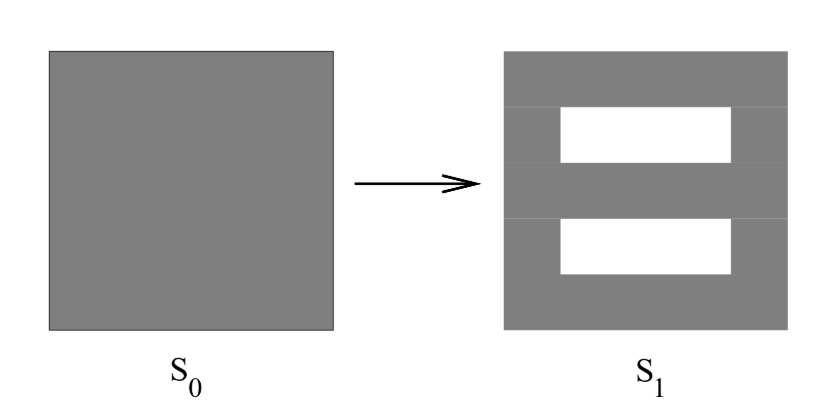
\includegraphics[width=0.5\textwidth]{Problem.png}
\end{center}
\vspace{-1em}
\begin{enumerate}
    \item[(a)] Draw the next iterate $S_2$ and describe the iteration rule in words.
    
    \item[(b)] Compute the dimension of the fractal object generated by repeatedly applying this rule. Use as many definitions or methods for dimension as you can.
\end{enumerate}

\paragraph{Solution}
\begin{enumerate}
    \item [(a)] The next iterate $S_2$ can be drawn by applying the following iteration rule:\\\\
    For each filled square, divide it into a 5 by 5 grid and remove the middle 3 squares from the second and fourth rows.\\\\
    Or in terms of matrix indices for each filled square:
\[
\begin{array}{c|ccccc}
 & j=1 & j=2 & j=3 & j=4 & j=5 \\ \hline
i=1 & (1,1) & (1,2) & (1,3) & (1,4) & (1,5) \\
i=2 & (2,1) & (2,2) & (2,3) & (2,4) & (2,5) \\
i=3 & (3,1) & (3,2) & (3,3) & (3,4) & (3,5) \\
i=4 & (4,1) & (4,2) & (4,3) & (4,4) & (4,5) \\
i=5 & (5,1) & (5,2) & (5,3) & (5,4) & (5,5)
\end{array}
\]
Remove:
\[(2,2), (2,3), (2,4), (4,2), (4,3), (4,4)\]
Then the next iterate subdivides each remaining square whose indices satisfy
\[
i\in\{1,3,5\}\quad \text{or}\quad j\in\{1,5\}.
\]
    \begin{center}
        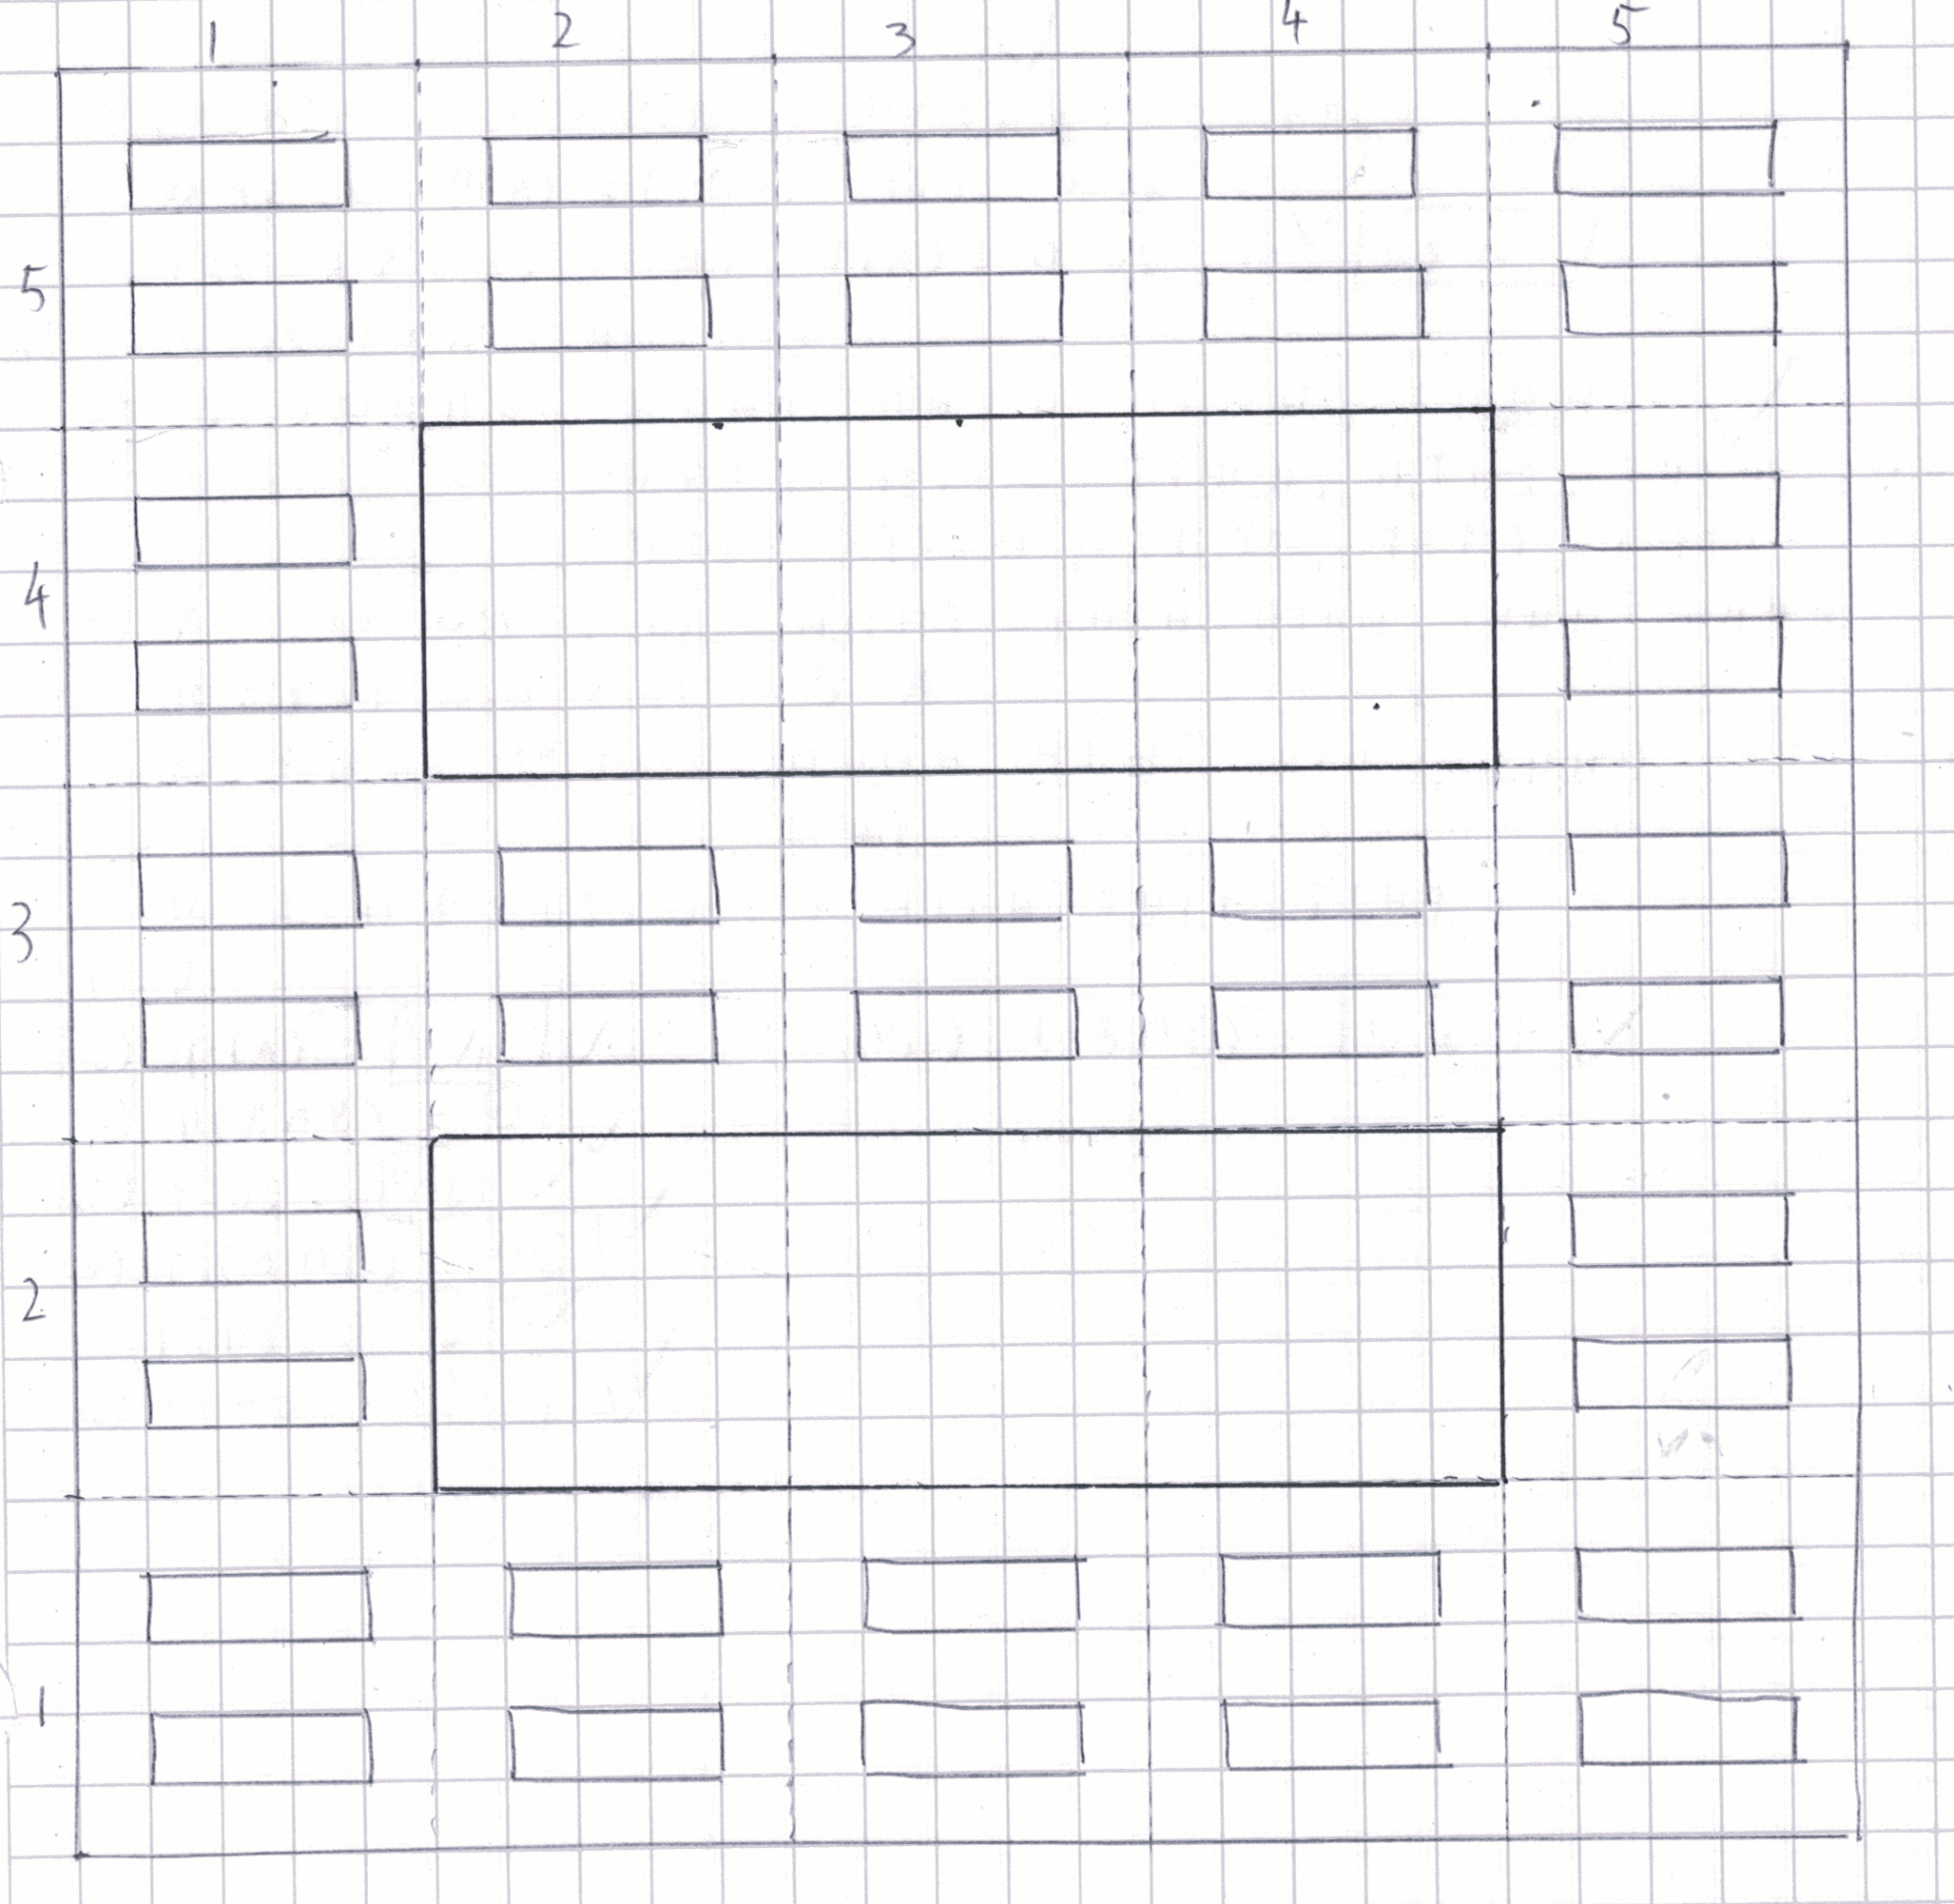
\includegraphics[width=0.8\textwidth]{S2.png}
    \end{center}
\end{enumerate}
Using the iteration rule, I tried to use Python to brute force the higher iterates, but it was too slow. With the help of ChatGPT, I was able to generate the next iterates using something called Kronecker products. The next iterates are shown below:
\begin{center}
    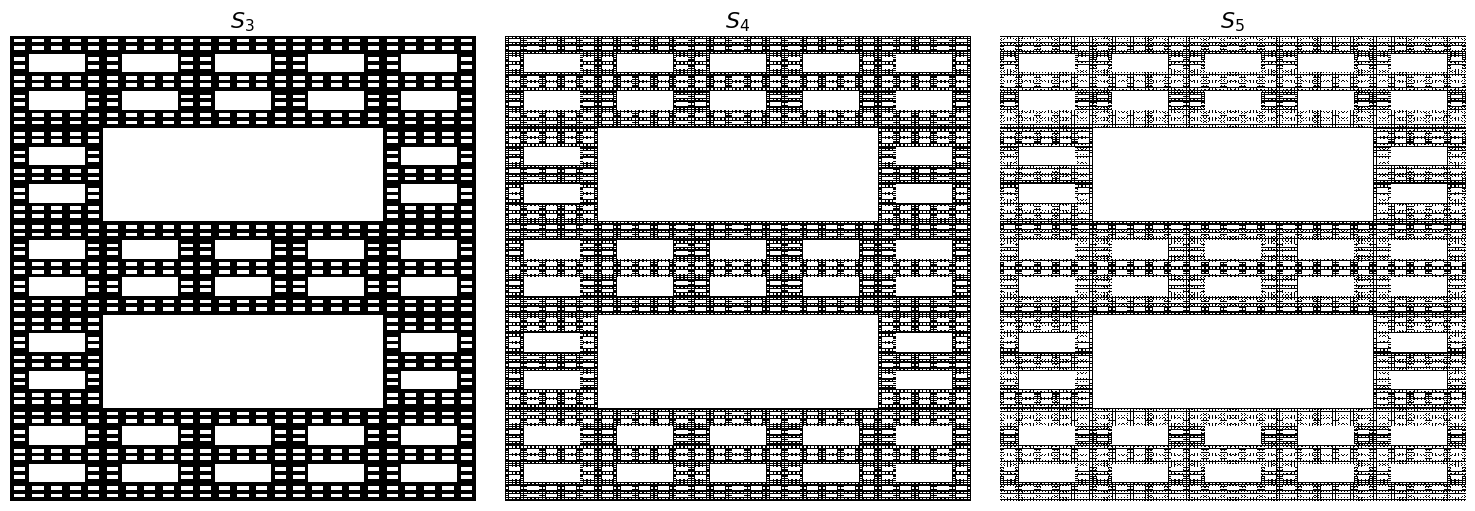
\includegraphics[width=\textwidth]{Iterates.png}
\end{center}
\begin{enumerate}
\item [(b)] \textbf{Similarity Dimension:}\\
 The similarity dimension $d_s$ is probably the most straightforward to compute. Since this is a self-similar fractal (made up of smaller copies of itself), we can use the formula:
\[d_s = \frac{\ln M}{\ln r}\]
Where $M$ is the number of self-similar copies contained in the fractal, and $r$ is the scaling factor.\\\\
In this case, 
\[M = 25 - 6 = 19 \quad \text{and} \quad r = 5\]
Thus, the similarity dimension is:
\[\boxed{d_s = \frac{\ln 19}{\ln 5} \approx 1.829}\]
\textbf{Box Dimension:}\\
The box dimension $d_b$ is a generalization of the similarity dimension for fractals that may not be strictly self-similar. It uses the number of boxes $N(\varepsilon)$ of edge length $\varepsilon$ needed to cover the fractal. The box dimension is defined as:
\[d_b = \lim_{\varepsilon \to 0} \frac{\ln N(\varepsilon)}{\ln(1/\varepsilon)}\]
For our fractal, suppose the edge length of the initial square in $S_0$ is $\varepsilon=1$ and is covered by one box. In the next iterate $S_1$, we have 19 boxes of edge length $\varepsilon=1/5$. In the next iterate $S_2$, we have $19^2$ boxes of edge length $\varepsilon=1/25$. Thus, we write a formula for $\varepsilon$ in terms of the iteration number $n$:
\[\varepsilon = \left(\frac{1}{5}\right)^n\]
and the number of boxes $N(\varepsilon)$ is:
\[N(\varepsilon) = 19^n\]
Substituting these into the box dimension formula, we have:
\[d_b = \lim_{\varepsilon \to 0} \frac{\ln N(\varepsilon)}{\ln(1/\varepsilon)} = \lim_{n \to \infty} \frac{\ln(19^n)}{\ln(5^n)} = \lim_{n \to \infty} \frac{n\ln(19)}{n\ln(5)} = \frac{\ln(19)}{\ln(5)}\]
Thus, the box dimension is:
\[\boxed{d_b = \frac{\ln 19}{\ln 5} \approx 1.829}\]
\textbf{Correlation Dimension}\\
The correlation dimension $d_c$ is a little bit different from the previous geometrical definitions. Instead, we populate the fractal with a large number of points and consider the number of points contained by a ball around a typical point $N_x(\varepsilon)$. The correlation dimension defines how fast the number of points contained in the ball grows as the ball grows. So generally, the correlation dimension is defined as:
\[C(\varepsilon) \propto \varepsilon^{d_c}\]
Where $C(\varepsilon)$ is just the average of $N_x(\varepsilon)$ over all points $x$.\\\\
Thus we can write the correlation dimension as the slope of the log-log plot of $C(\varepsilon)$ vs $\varepsilon$:
\begin{center}
    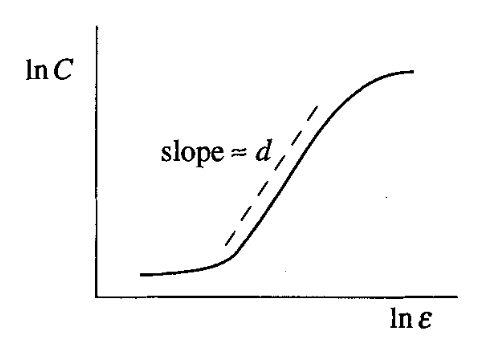
\includegraphics[width=0.4\textwidth]{Correlation.png}
\end{center}
For our fractal, we can approximate the correlation dimension by comparing the number of points to the area of the fractals. We know from the previous parts that as we scale down the fractal by a factor of $5$, we "zoom in" on one of the $19$ self-similar copies. Thus, we can write:
\[C\left(\frac{\varepsilon}{5}\right) = \frac{1}{19} C(\varepsilon)\]
Since $C(\varepsilon) \propto \varepsilon^{d_c}$, we can write:
\[C(\varepsilon) = K \varepsilon^{d_c}\]
Where $K$ is some constant. Substituting for $\varepsilon/5$ into the equation, we have:
\begin{eqnarray*}
    C\left(\frac{\varepsilon}{5}\right)&=&K\left(\frac{\varepsilon}{5}\right)^{d_c}\\
    &=&K\varepsilon^{d_c}\left(\frac{1}{5}\right)^{d_c}\\
    &=&C(\varepsilon)\left(\frac{1}{5}\right)^{d_c} \quad \text{(since $C(\varepsilon) = K \varepsilon^{d_c}$)}\\
\end{eqnarray*}
Now we can equate this to the previous equation:
\[C\left(\frac{\varepsilon}{5}\right) =C(\varepsilon)\left(\frac{1}{5}\right)^{d_c} = \frac{1}{19} C(\varepsilon) \]
\[\implies 5^{d_c} = 19\]
\[\implies d_c \ln(5) = \ln(19)\]
\[\implies d_c = \frac{\ln(19)}{\ln(5)} = \boxed{1.829}\]
\end{enumerate}

\end{document}